\documentclass{article}

\usepackage{graphicx}
\usepackage{geometry}
\usepackage{amsmath}
\usepackage{enumerate}
\usepackage{natbib}

\geometry{top=1in,
		left=0.5in,
		right=0.5in,
		bottom=1in}
	
\newcommand{\bone}{\mathbf{1}}
\newcommand{\bphi}{\boldsymbol{\phi}}
\newcommand{\sD}{\mathcal{D}}
\newcommand{\bm}{\mathbf{m}}
\newcommand{\bC}{\mathbf{C}}
\newcommand{\bA}{\mathbf{A}}
\newcommand{\btheta}{\boldsymbol{\theta}}
\newcommand{\bF}{\mathbf{F}}
\newcommand{\bG}{\mathbf{G}}
\newcommand{\bW}{\mathbf{W}}
\newcommand{\ba}{\mathbf{a}}
\newcommand{\bR}{\mathbf{R}}
	
\title{West \& Harrison Chapter 10, Problem 7}
\author{The Dans}
\date{Thursday, March 16, 2017}

\begin{document}
	\maketitle
	
	The quarterly sales and cost index of a confectionary product are given as  %in figure \ref{fig:data}.
%	\begin{figure}[h]
%		\centering
%		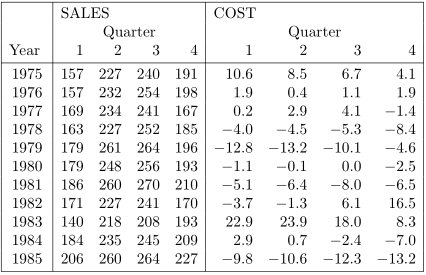
\includegraphics[width=0.4\linewidth]{Data}
%		\caption{The data associated with the problem}
%		\label{fig:data}
%	\end{figure}

	\begin{center}
		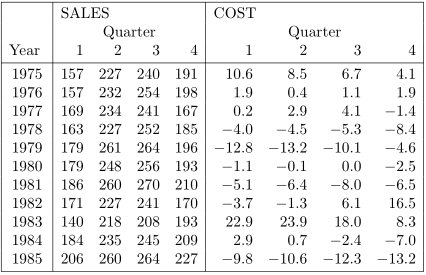
\includegraphics[width=0.5\linewidth]{Data}
	\end{center}

	The goal is to fit a DLM to the sales with first-order polynomial, regression on cost, and full seasonal components. Based on previous information, 
	\begin{itemize}
		\item the underlying level of the series when cost is zero is 220 with a nominal standard error of 15
		\item the regression coefficient of cost is estimated as -1.5 with a standard error of about 0.7
		\item the seasonal factors for the four quarters of the first year are expected to be -50, 25, 50, -25, with nominal standard errors of 25, 15, 25, and 15, respectively
		\item the trend, regression, and seasonal components are initially assumed to be uncorrelated
		\item the observational variance is estimated as 100, with initial degrees of freedom of 12
	\end{itemize}
	Using this information, we are to analyze the series along the following lines:
	\begin{enumerate}[(a)]
		\item \textbf{Using the information provided for the seasonal factors above, apply Theorem 8.2 to derive the appropriate initial prior that satisfies the zero-sum constraint.}
		
		\textit{Theorem 8.2: Imposing the constraint $\bone'\bphi = 0$ on the prior $(\bphi_0|\sD_0^*) \sim \text{N}(\bm_0^*,\bC_0^*)$ and writing $U = \bone'\bC_0^*\bone$ and $\bA = \bC_0^*\bone/U$ gives the revised joint prior}
		\begin{align*}
			(\bphi_0|\sD_0) & \sim \text{N}(\bm_0,\bC_0),\\
			\bm_0 = \bm_0^* & - \bA\bone'\bm_0^*,\\
			\bC_0 = \bC_0^* & - \bA\bA'U.
		\end{align*} 
		Using the given information for the seasonal components,
		\begin{align*}
			\bm_0^* & = (-50,25,50,-25)' &
			\bC_0^* & = \begin{pmatrix}
				625 & 0 & 0 & 0 \\
				0 & 225 & 0 & 0 \\
				0 & 0 & 625 & 0 \\
				0 & 0 & 0 & 225
			\end{pmatrix}.
		\end{align*}
		Applying Theorem 8.2 yields
		\begin{align*}
			U & = 1700 \\ A & = (0.3676471, 0.1323529, 0.3676471, 0.1323529)' \\
			\bm_0^s & = (-50,  25,  50, -25)' \\
			\bC_0^s & = \begin{pmatrix}
			395.22 & -82.72 & -229.78 & -82.72 \\ 
			-82.72 & 195.22 & -82.72 & -29.78 \\ 
			-229.78 & -82.72 & 395.22 & -82.72 \\ 
			-82.72 & -29.78 & -82.72 & 195.22 \\ 
			\end{pmatrix}.
		\end{align*}
		This leads to the initial prior satisfying the zero-sum constraint for the seasonal components to be $(\bphi_0|\sD_0) \sim \text{N}(\bm_0^s,\bC_0^s)$. Given a state vector $\btheta_t = (\theta_{1,t},\theta_{2,t},\phi_{1,t},\ldots,\phi_{4,t})'$, the initial prior for the DLM is of the form $(\btheta_0|\sD_0) \sim \text{N}(\bm_0,\bC_0)$, where
		\begin{align*}
			\bm_0 & = (220,-1.5, -50,  25,  50, -25)' \\
			\bC_0 & = \begin{pmatrix}
			225.00 & 0.00 & 0.00 & 0.00 & 0.00 & 0.00 \\ 
			0.00 & 0.49 & 0.00 & 0.00 & 0.00 & 0.00 \\ 
			0.00 & 0.00 & 395.22 & -82.72 & -229.78 & -82.72 \\ 
			0.00 & 0.00 & -82.72 & 195.22 & -82.72 & -29.78 \\ 
			0.00 & 0.00 & -229.78 & -82.72 & 395.22 & -82.72 \\ 
			0.00 & 0.00 & -82.72 & -29.78 & -82.72 & 195.22 \\ 
			\end{pmatrix}.
		\end{align*}
		
		\item \textbf{Identify the full initial prior quantities for the 6-dimensional state vector $\btheta_1$ and the observational variance $V$. Write down the defining quantities $\ba_1,\bR_1,n_0$, and $S_0$ based on the above initial information.}
		
		The DLM model in this case is defined as $\{ \bF_t, \bG,V,\bW_t \}$, with 
		\begin{align*}
			\bF_t & = (1,\text{Cost}_t,1,0,0,0)' &
			\bG & = \begin{pmatrix}
			1 & 0 & 0 & 0 & 0 & 0 \\
			0 & 1 & 0 & 0 & 0 & 0 \\
			0 & 0 & 0 & 1 & 0 & 0 \\
			0 & 0 & 0 & 0 & 1 & 0 \\
			0 & 0 & 0 & 0 & 0 & 1 \\
			0 & 0 & 1 & 0 & 0 & 0 \\
			\end{pmatrix}.
		\end{align*}
		Using this information,
		\begin{align*}
			\ba_1 & = \bG\bm_0 = (220,  -1.5,  25,  50, -25, -50)' \\
			\bR_1 & = \bG\bC_0\bG' + \bW_t = \begin{pmatrix}
			225.00 & 0.00 & 0.00 & 0.00 & 0.00 & 0.00 \\ 
			0.00 & 0.49 & 0.00 & 0.00 & 0.00 & 0.00 \\ 
			0.00 & 0.00 & 195.22 & -82.72 & -29.78 & -82.72 \\ 
			0.00 & 0.00 & -82.72 & 395.22 & -82.72 & -229.78 \\ 
			0.00 & 0.00 & -29.78 & -82.72 & 195.22 & -82.72 \\ 
			0.00 & 0.00 & -82.72 & -229.78 & -82.72 & 395.22 
			\end{pmatrix}  + \bW_t\\
			n_0 & = 12 \\
			S_0 & = 100.
		\end{align*}
		Therefore, $(\btheta_1|\sD_0) \sim \text{T}_{12}(\ba_1,\bR_1)$ and $(V|\sD_0) \sim \text{Inverse Gamma}(n_0/2,d_0/2)$, where $d_0 = n_0S_0 = 1200$.
		
		\item \textbf{Use three discount factors to structure the evolution matrices of the model: $\delta_T$ for the constant intercept term, $\delta_R$ for the regression coefficient, and $\delta_S$ for the seasonal factors. Consider initially the values $\delta_T = \delta_S = 0.9$ and $\delta_R = 0.98$. Fit the model and perform the retrospective, filtering calculations to obtain filtered estimates of the state vector and all model components over time.}
		
		The filtered estimates of each component of the state vector are shown in figure \ref{fig:filteredestimates}. The one-step ahead forecast and 95\% confidence interval can be seen in figure \ref{fig:forecastdist}.
		
		\begin{figure}
			\centering
			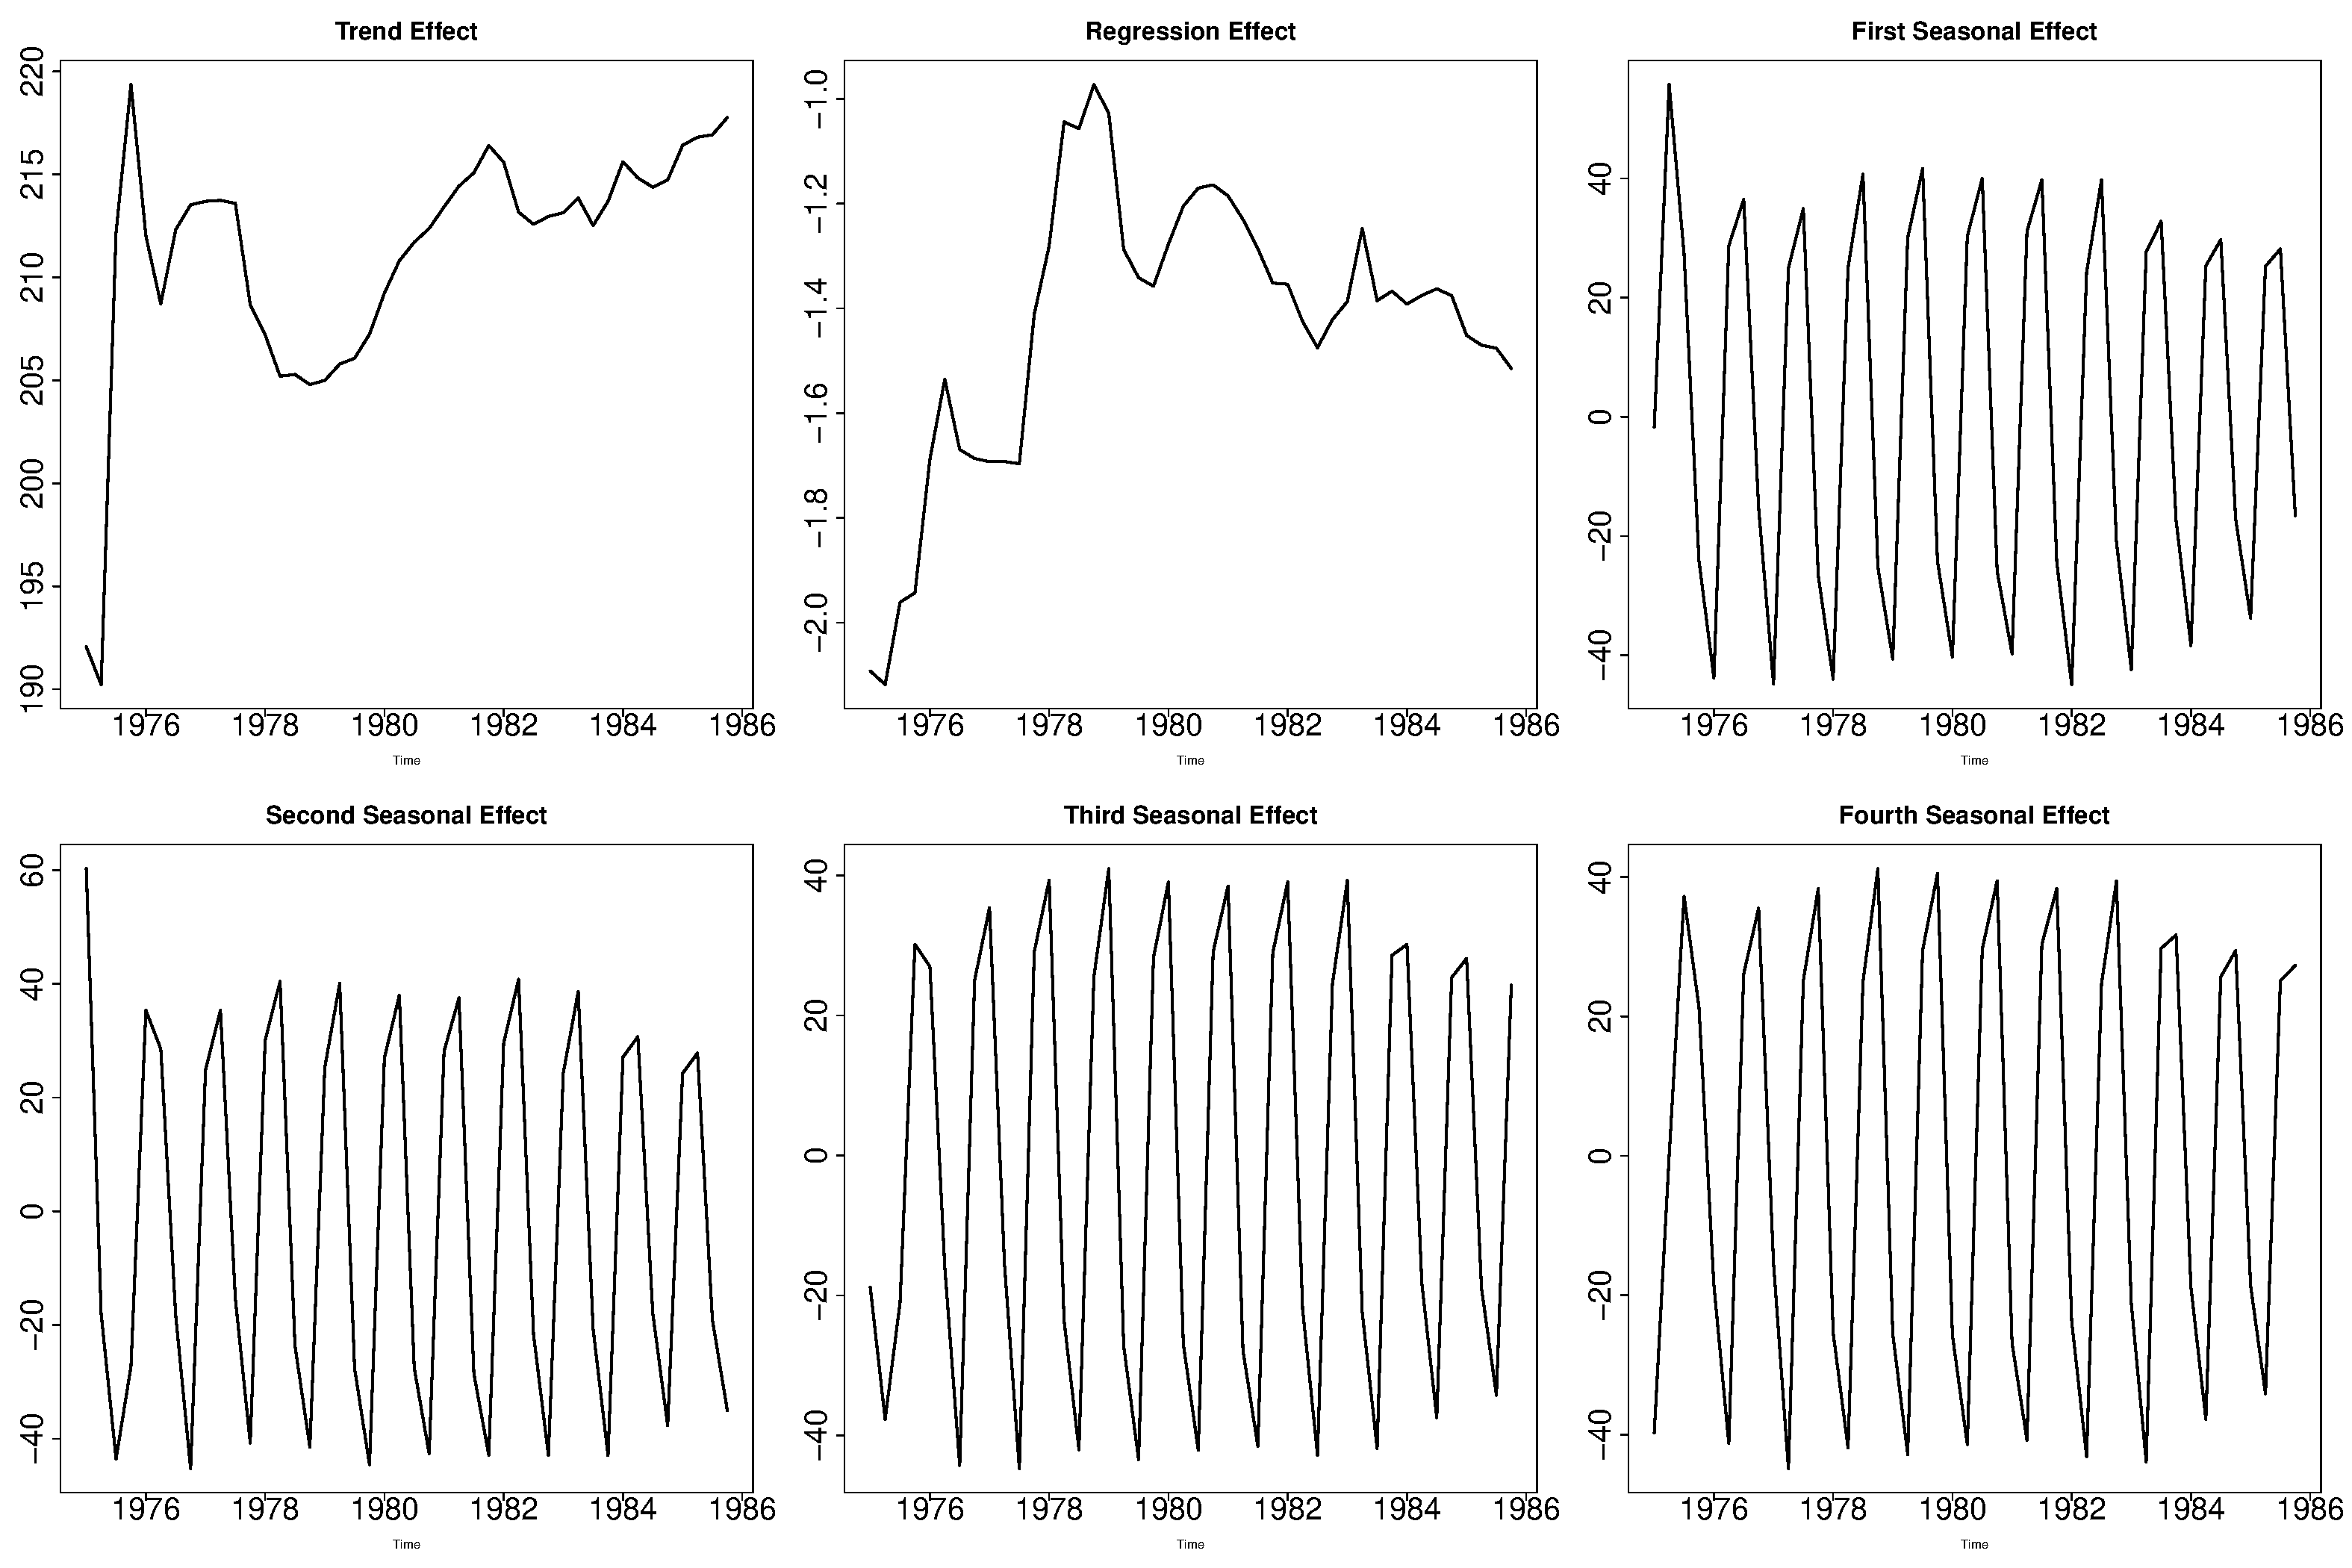
\includegraphics[width=\linewidth]{Filteredestimates}
			\caption{Filtered estimates for all components of the state vector}
			\label{fig:filteredestimates}
		\end{figure}
		
		\begin{figure}
			\centering
			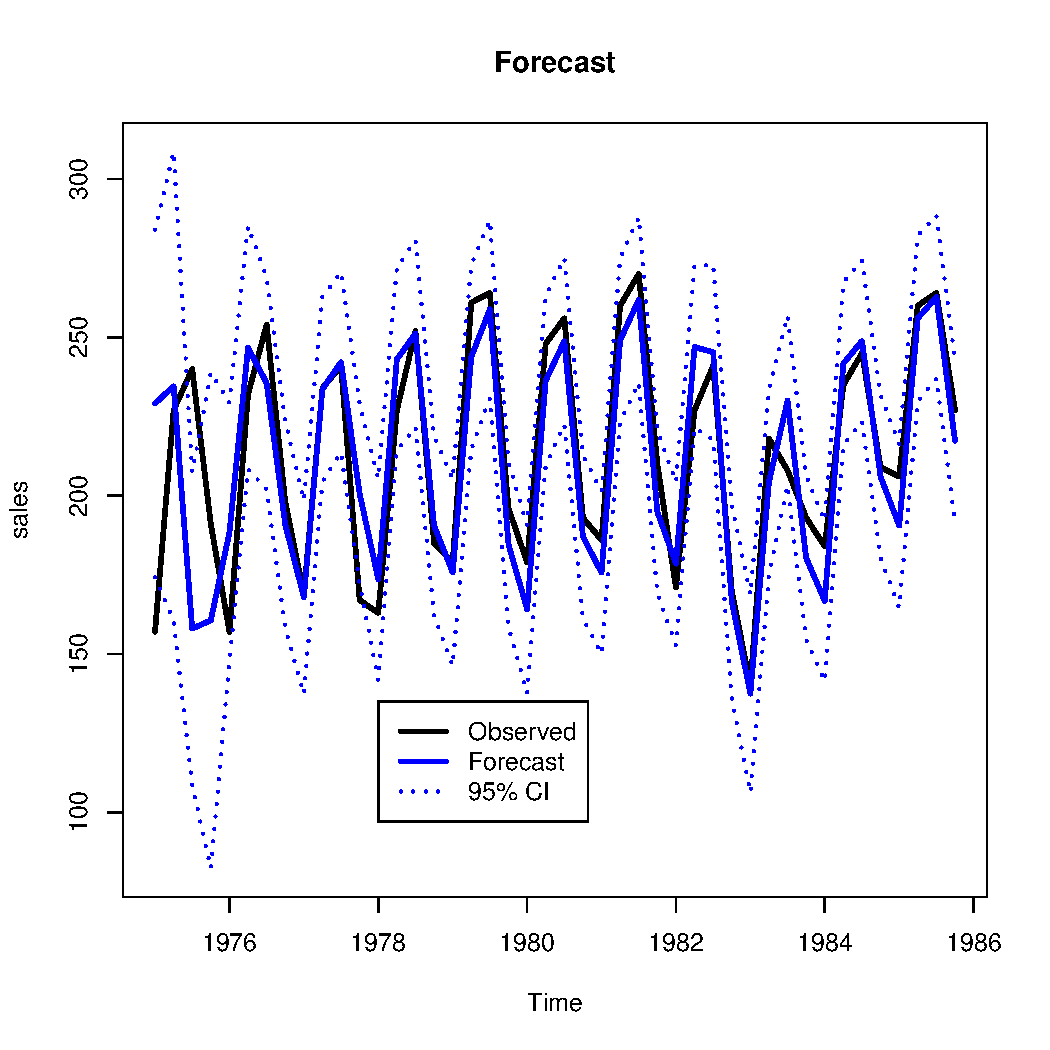
\includegraphics[width=0.7\linewidth]{ForecastDist}
			\caption{One-step ahead forecast estimate and 95\% confidence interval}
			\label{fig:forecastdist}
		\end{figure}
		
		\item \textbf{Based on this analysis, verify the findings in \cite{WHP1987b} to the effect that the regression parameter on Cost is, in retrospect, rather stable over time.}
		
		Figure \ref{fig:costandregressionparm} shows the values for Cost relative to the estimates of the regression parameter. Based on this plot, it does not appear that the values for the regression parameter change very much over time, always hovering between -1 and -2.
		
		\begin{figure}
			\centering
			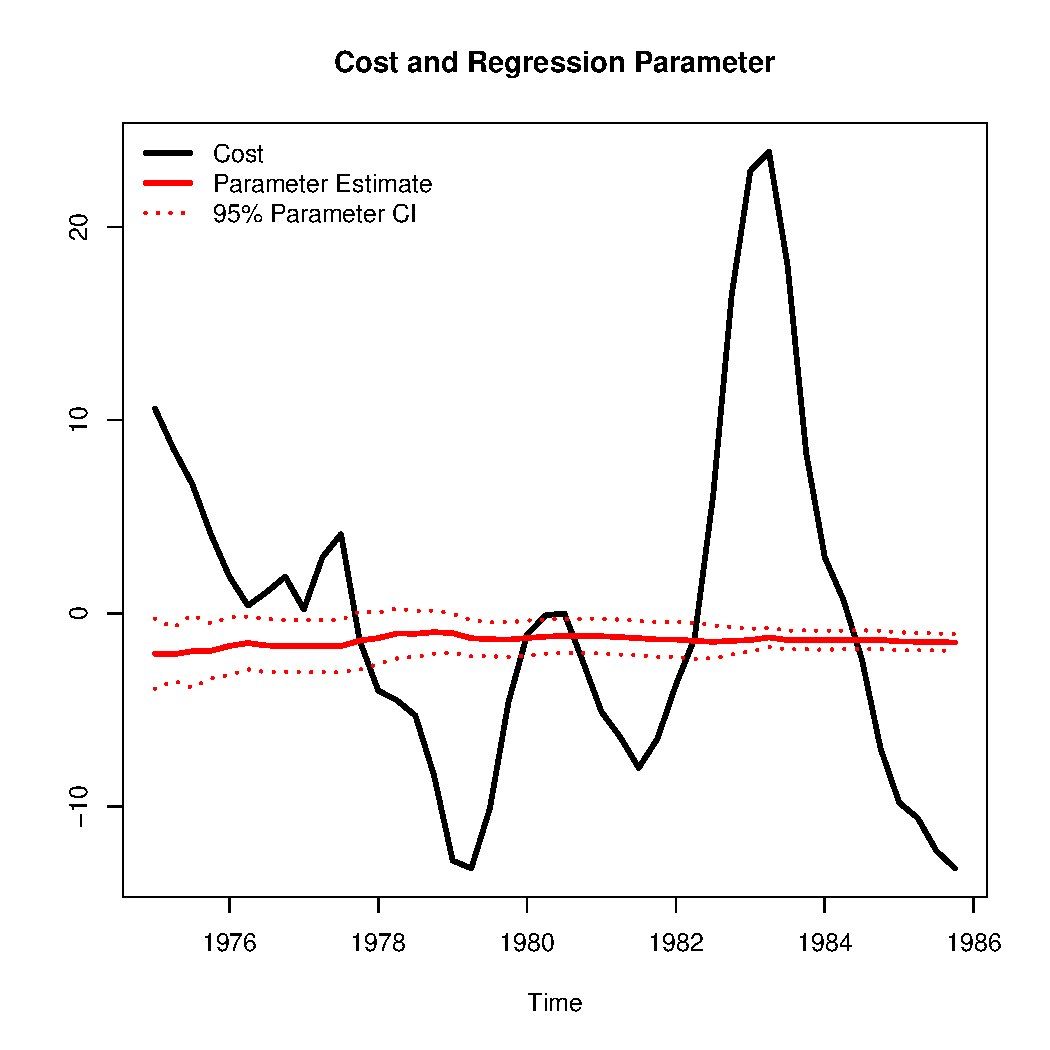
\includegraphics[width=0.7\linewidth]{CostandRegressionParm}
			\caption{Plot of the observed cost and a summary of the distribution of the regression parameter}
			\label{fig:costandregressionparm}
		\end{figure}
		
		\item \textbf{Produce step ahead forecasts from the end of the data in the fourth quarter of 1985 for the next three years. The estimated values of Cost to be used in forecasting ahead are given by}
		\begin{center}
			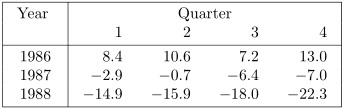
\includegraphics[width=0.5\linewidth]{CostFuture}
		\end{center}
		
	\end{enumerate}
	
\bibliography{WHCh10Pr7}
\bibliographystyle{plainnat}
	
\end{document}